\documentclass[11pt]{article}

\usepackage[utf8]{inputenc}
\usepackage[T1]{fontenc}
\usepackage[margin=1.1in]{geometry}
\usepackage{amsmath,amssymb,amsthm}
\usepackage{mathtools}
\usepackage{enumitem}
\usepackage{tikz}
\usetikzlibrary{arrows.meta,positioning,decorations.pathreplacing,calc}
\usepackage[hidelinks]{hyperref}
\usepackage{xcolor}

% Todo macro for placeholders to be filled in later phases.
\newcommand{\todo}[1]{{\color{red}\textbf{[TODO: #1]}}}

% Theorem environments.
\newtheorem{theorem}{Theorem}[section]
\newtheorem{proposition}[theorem]{Proposition}
\newtheorem{lemma}[theorem]{Lemma}
\newtheorem{corollary}[theorem]{Corollary}

\theoremstyle{definition}
\newtheorem{definition}[theorem]{Definition}
\newtheorem{example}[theorem]{Example}

\theoremstyle{remark}
\newtheorem{remark}[theorem]{Remark}
\newtheorem{notation}[theorem]{Notation}

% Notation macros.
\newcommand{\Kp}{\mathrm{Kp}}
\newcommand{\NT}{\mathrm{NT}}
\newcommand{\Sing}{\mathrm{Sing}}
\newcommand{\Chain}{\mathrm{Chain}}
\newcommand{\MB}{\mathrm{MB}}
\newcommand{\TM}{\mathrm{TM}}
\newcommand{\KK}{\mathbb{K}}
\newcommand{\Z}{\mathbb{Z}}
\newcommand{\Zn}{\Z_{\geq 0}}
\newcommand{\g}{\mathfrak{g}}
\newcommand{\Uq}{U_q(\g)}
\newcommand{\Uqm}{U_q^-(\g)}
\newcommand{\Uiota}{U^\imath}
\newcommand{\Cmid}{\mathcal{C}}
\newcommand{\Csing}{\mathcal{C}_{\mathrm{sing}}}
\newcommand{\TT}{\mathcal{T}}
\newcommand{\br}{\mathrm{br}}
\newcommand{\eps}{\varepsilon}
\newcommand{\labr}[1]{{)}_{#1}}
\newcommand{\labl}[1]{{(}_{#1}}
\DeclareMathOperator{\sgn}{sgn}

\title{A tensor product rule for $\imath$-crystals across the short--long edge in type B}
\author{Rick}
\date{\today}

\begin{document}
\maketitle

\begin{abstract}
We prove a type-uniform tensor product decomposition for the Kostant-partition $\imath$-crystal
$\Kp(\infty)$ of type $B_n$, $n \geq 2$, restricted to the short-simple $\imath$-coideal generator
$B_n$. The decomposition is
\[
\Kp(\infty)\big|_{B_n} \;\cong\; \bigotimes_{a=1}^{n-1} \Cmid_a \;\otimes\; \Csing
\]
as $\imath$-crystals, where each chain factor $\Cmid_a$ is a new rank-three building block
encoding the short--long Cartan entry $a_{n-1,n} = -2$ via doubled interior brackets, and the
singleton factor $\Csing \cong \KK[B_n]$ matches Watanabe's split-node $\imath$-crystal verbatim.
The on-slice $e_n^2$ catalog has $n(2n-1)$ entries with the three-class decomposition
\[
n(2n-1) \;=\; 3(n-1) \;+\; 2(n-1)(n-2) \;+\; (2n-1),
\]
where the three summands count intra-chain, cross-chain, and singleton-involving pairs of
primitive operators. The rule extends Watanabe (arXiv:2110.07177, Proposition~5.1.1) past
the simply-laced quasi-split restriction $(\mathrm{S1})$--$(\mathrm{S3})'$ in the unique
case it omits, the short--long edge of type $B_n$.
\end{abstract}

\tableofcontents

%==============================================================================
\section{Introduction}
%==============================================================================

\subsection{Statement of the problem}

Quantum symmetric pairs $(\Uq, \Uiota)$ generalise enveloping algebras of symmetric pair Lie
algebras to the quantum setting. Their highest-weight representation theory carries the same
non-trivial combinatorial shadow that Kashiwara's crystal basis theory gives for $\Uq$ itself.
Watanabe \cite{Watanabe2107,Watanabe2110} initiated a systematic crystal theory for $\imath$-quantum
groups by constructing per-node $\imath$-crystals and a tensor product rule that propagates the
$\imath$-coideal generators across simply-laced edges of the Satake diagram.

The construction of \cite{Watanabe2110} has one structural limitation. The tensor product rule
is conditional on a triple of axioms $(\mathrm{S1})$--$(\mathrm{S3})'$ that hold precisely when
the relevant off-diagonal Cartan entry satisfies $a_{ij} \in \{0, -1\}$, i.e., on simply-laced
edges. In the BDI family (type B, split), every node is split and so per-node objects come
from \cite[\S4.1]{Watanabe2110} uniformly, and every long--long edge $a_{a,b} = -1$ with
$1 \leq a, b < n$ is handled by \cite[Prop.~5.1.1]{Watanabe2110}. The unique remaining edge
is the short--long edge $a_{n-1,n} = -2$, which is excluded by $(\mathrm{S1})$--$(\mathrm{S3})'$
and is therefore the unique obstacle to a complete crystal-theoretic description of $\Kp(\infty)$
for $B_n$ under the full $\Uiota$-action.

This paper closes that gap. We construct a new rank-three building block --- the \emph{chain
factor} $\Cmid_a$ --- and prove that the short-simple restriction of $\Kp(\infty)|_{B_n}$
factorises as a tensor product of $n - 1$ chain factors and one singleton factor, with an
explicit bracket-concatenation rule. The construction is type-uniform in $n$ and matches the
empirically verified $e_n^2$ catalog at $B_2, B_3, B_4, B_5$.

\subsection{Prior work}

We outline the immediate predecessors.

\medskip
\noindent\textbf{Watanabe, type AI and quasi-split.}
Watanabe \cite{Watanabe2107} constructs an $\imath$-crystal structure on $V(\lambda)$ at type AI,
with $\imath$-Kashiwara operators $\widetilde B_i$ satisfying a commutation relation $\widetilde
B_i \widetilde B_j = \widetilde B_j \widetilde B_i$ whenever $|i - j| > 1$. There is no braid
relation; the construction is per-node plus pairwise commutation.

In \cite{Watanabe2110}, Watanabe extends to the quasi-split setting and identifies axioms
$(\mathrm{S1})$--$(\mathrm{S3})'$ on the Satake diagram under which $\imath$-Kashiwara
operators propagate via Kashiwara signature rules across edges. These axioms enforce $a_{ij}
\in \{0, -1\}$ on every off-diagonal entry: the simply-laced condition. The split case (where
$\tau = \mathrm{id}$ and every node has $a_{i,\tau(i)} = 2$) yields per-node objects $U^i_i =
\KK[B_i]$ and a tensor product rule across simply-laced edges. The type-BDI short--long edge
$a_{n-1,n} = -2$ is omitted.

\medskip
\noindent\textbf{Algebra-level type-B foundations.}
On the algebraic side, the relevant $\imath$-quantum group theory is in place. Chen, Lu and
Wang \cite{CLW} and Jian, Luo and Wu \cite{JLW} construct Lyndon-word bases and PBW-type
generating sets for split $\imath$-quantum groups including type BDI. The relations are
controlled by the iSerre identities of Letzter, Kolb, and Bao--Wang \cite{BaoWang}. The
combinatorial structure at the algebra level is therefore not the obstacle. The obstacle is
that no crystal-level analogue of these algebra-level constructions has been written down for
type BDI in full generality; the survey of Wang \cite{Wang2024Survey} notes the gap explicitly.

\medskip
\noindent\textbf{Adjacent crystal-theoretic frameworks.}
Two adjacent recent works frame the territory. Azenhas and Torres \cite{AzenhasTorres} construct
an evacuation involution on type-B Kashiwara--Nakashima tableaux via a virtualisation argument,
giving cactus-group structure at the Littelmann-path level. Their construction outputs an
involution on $B(\lambda)$, which is a different combinatorial register from ours --- the
present paper outputs a tensor product decomposition of $\Kp(\infty)|_{B_n}$ as an
$\imath$-crystal.

Zhang \cite{Zhang2509} establishes a bridge between iquantum AIII weight spaces and type-B
Hecke modules via Wang--Zhang relative braid group symmetries. Zhang's bridge is at the
algebraic level (generic $q$) and operates between full weight spaces, not catalog entries;
no crystal-level descent is given. The present paper is the type-BDI crystal-level counterpart
to that algebraic AIII--Hecke correspondence.

\medskip
\noindent\textbf{Categorification at generic $q$.}
Brundan, Wang and Webster \cite{BWB2505} construct a categorification of quasi-split
$\imath$-quantum groups in all symmetric types, with type AIII as their worked example.
The phrase ``all symmetric types'' refers there to the ambient Cartan matrix being
symmetric, not to a Satake-type label; the BDI Satake type studied here is not in their
immediate scope. Their construction lives at the 2-categorification level at generic $q$
and over an integer form, whereas the present paper operates at the crystal level
($q = 0$) for BDI. The two pictures are orthogonal; a future meeting point would require
a BDI 2-categorification to be constructed in the BWB framework, which is not currently
available.

\medskip
\noindent\textbf{Crystal-level type-B combinatorics at a single node.}
Park and Jung \cite{ParkJung2507} give a crystal-theoretic description of the Kimura--Oya
quantum twist automorphisms on the quantum unipotent coordinate rings, with explicit
type-$B_n$ combinatorics at the spin minuscule node via shifted Young diagrams. Their
work is not framed in $\imath$-quantum or QSP language and is adjacent rather than
directly comparable, but it furnishes a useful precedent for crystal-level combinatorial
control over a single type-B node and shows that the spin-minuscule register is amenable
to clean combinatorial encoding.

\subsection{Main theorem (informal)}

For $\g$ of type $B_n$ with $n \geq 2$, let $B_n = F_n + \varsigma_n E_n K_n^{-1}$ be the short-simple
$\imath$-coideal generator. The Kostant partition crystal $\Kp(\infty)$ of $\Uqm$ is the
$\Zn$-lattice with coordinates indexed by positive roots $\Phi^+(B_n)$. Restricting to the
$B_n$-action and discarding the trivial factors coming from roots not in any $\alpha_n$-string,
the resulting $\imath$-crystal factorises as
\[
\bigotimes_{a=1}^{n-1} \Cmid_a \;\otimes\; \Csing,
\]
where $\Cmid_a$ is the chain factor associated to the $\alpha_n$-string $\Chain(a) = \{E_a -
E_n,\; E_a,\; E_a + E_n\}$ and $\Csing$ is the singleton factor associated to $\{E_n\}$.
The tensor-product bracket is the concatenation of per-factor brackets in convex chain order
followed by the singleton block; cancellation propagates across factor boundaries by the
standard Kashiwara signature rule. The on-slice $e_n^2$ catalog has size $\binom{2n}{2} =
n(2n-1)$, decomposing as
\[
\underbrace{3(n-1)}_{\text{intra-chain}} \;+\; \underbrace{2(n-1)(n-2)}_{\text{cross-chain}} \;+\;
\underbrace{(2n-1)}_{\text{singleton-involving}}.
\]
The three classes correspond exactly to the three types of factor incidence of a pair of
primitive operators: both in the same chain factor, in two distinct chain factors, or at least
one in the singleton factor.

The formal statement is Theorem \ref{thm:main}. The key new ingredient is the chain factor
$\Cmid_a$ with bracket block $\labr{E_a}^M\, \labl{E_a - E_n}^{2B}\, \labr{E_a + E_n}^{2T}\,
\labl{E_a}^M$. The doubled inner exponents $2B, 2T$ are the bracket-level expression of the
short--long Cartan entry $a_{n-1,n} = -2$. This is the new building block beyond the rank-one
per-node objects of \cite[\S4.1]{Watanabe2110}.

\subsection{Strategy of proof}

The proof has four phases.

\begin{itemize}[leftmargin=2em]
  \item[\textbf{Phase A: Chain factor uniformity.}] We define $\Cmid_a$ and show that its
    bracket block depends only on local Cartan data and chain position, hence is structurally
    the same for every $a \in \{1, \ldots, n-1\}$ and every $n \geq 2$. Only the labels
    differ.
  \item[\textbf{Phase B: Tensor product as $\imath$-crystal.}] We define
    $\TT_n = \bigotimes_a \Cmid_a \otimes \Csing$ and identify it with $\Kp(\infty)|_{B_n}$
    via the CST bracketing of the short simple. The identification is on the nose: the
    tensor-product bracket is exactly the CST bracketing read as a string concatenation.
  \item[\textbf{Phase C: Catalog factor-by-factor.}] We realise each of the $\binom{2n}{2}$
    catalog entries by an explicit Kostant-partition witness supported on at most two factors,
    with bracket-level arguments uniform in the chain indices. This step contains the
    substantive combinatorics; cross-chain entries between non-adjacent chains work
    identically to adjacent ones because intermediate chains contribute no bracket symbols
    when given zero multiplicity.
  \item[\textbf{Phase D: Type-uniformity wrap.}] All steps in A--C are uniform in $n$, with
    arithmetic-only dependence on the rank. Phase D collects the pieces.
\end{itemize}

The present paper develops Section \ref{sec:prelim} (preliminaries), states and proves Phase A
in Section \ref{sec:main}, and defers Phases B, C, D to Sections \ref{sec:phaseB},
\ref{sec:phaseC}, \ref{sec:phaseD}.

\subsection{Downstream picture}\label{ssec:downstream}

Once the short--long tensor product rule is established at the crystal level, the natural
downstream programme is operationalisation for quantum Littlewood--Richardson maps in BDI.
The corresponding picture in type AII has already been laid down. Naito, Suzuki and
Watanabe \cite{NSW2024} reproved the Naito--Sagaki conjecture as a branching rule for
$\imath$-crystals of type AII, and
Azenhas's two recent papers \cite{Azenhas2603,Azenhas2604} develop the quantum
Littlewood--Richardson map of \cite{Watanabe2110} at the recording-tableau level:
\cite{Azenhas2603} studies the recording tableaux of the quantum LR map together with the
orthogonal transpose symmetry map and the computation of highest-weight tableaux, and
\cite{Azenhas2604} introduces the slack data of these recording tableaux to characterise
the inverse of the quantum LR map. Theorem~\ref{thm:main} is the
crystal-level input that enables the type-B/D analog of this programme: a
tensor-product-rule-driven combinatorial model for $\imath$-quantum BDI Littlewood--Richardson
maps. We do not pursue this here; the present paper supplies only the crystal-theoretic
foundation.

\subsection{Organisation}

Section \ref{sec:prelim} fixes notation, recalls the necessary Kashiwara crystal background,
sketches the $\imath$-crystal extension of \cite{Watanabe2107,Watanabe2110}, introduces the
bracket alphabet, defines the slice $K_p(\infty)$ relevant to the short simple, and writes
down the chain and singleton factors. Section \ref{sec:main} states the main theorem and
proves Phase A. Sections \ref{sec:phaseB}--\ref{sec:phaseD} contain Phases B--D.

\subsection{Scope of the bracket framework}\label{ssec:scope}

We close the introduction with a remark on the structural scope of the chain-factor
construction; Figure~\ref{fig:bracket-trichotomy} summarises the trichotomy of regimes
discussed below.

\begin{remark}[Natural scope of the bracket framework]\label{rmk:scope}
The bracket framework underlying the chain factor $\Cmid_a$ has a structurally-determined
ceiling at off-diagonal Cartan entry $|a| \leq 2$. The present paper sits at this ceiling,
not at an arbitrary intermediate point: the same mechanism --- chain interior length
governs the form of the mid-bracket framing --- explains both Watanabe's stopping point at
$|a| \leq 1$ and ours at $|a| = 2$.

Concretely, for a Cartan entry $|a_{ji}| = m$, the relevant $\alpha_i$-string through the
chosen short root has length $m + 1$, with $m - 1$ \emph{interior} positions:
\begin{itemize}[leftmargin=2em]
  \item $m \in \{0, 1\}$ (simply-laced, Watanabe's case
    \cite[Prop.~5.1.1]{Watanabe2110}). The chain has no interior position, no mid-bracket
    framing is needed, and the rank-one per-node objects of \cite[\S4.1]{Watanabe2110}
    glue across the edge by the standard signature rule.
  \item $m = 2$ (the present paper; the short--long edge of $B_n$, and by symmetric
    relabelling the analogous edges of $C_n$ and $F_4$). The chain has exactly one
    interior position --- the mid root $E_a$ with $\langle E_a, \alpha_n^\vee\rangle = 0$
    --- and is framed by the unique mid-bracket pair $\labr{E_a}^M \cdots \labl{E_a}^M$
    of (\ref{eq:chain-bracket-block}). The doubled exponents $2B, 2T$ on the inner
    sub-blocks encode $|a| = 2$.
  \item $m \geq 3$ (the triple edge of $G_2$, and hyperbolic generalisations). The chain
    has two or more interior positions with mixed (non-zero) $\alpha^\vee$-pairings, and
    no clean bracket framing of the present form exists.
\end{itemize}

The $|a| \geq 3$ obstruction is genuine, not an artefact of method. A short computational
verification carried out for the present project tested the nine natural candidate
bracket layouts for the chain factor at $G_2$ and confirmed that none of them satisfies
Kashiwara injectivity for the $\imath$-coideal generator. The specific obstructing
witnesses can be exhibited at $G_2$ between the partitions $\pi_A = \beta_1 + \beta_3$
(low-mid plus top of the length-four chain through $\alpha_1$) and $\pi_B = 2\beta_2$
(twice the high-mid root): in any candidate layout that respects the per-root contribution
rule, both partitions admit an $f_1$-action landing on the same partition $\beta_2 +
\beta_3$, violating injectivity. We do not include the computational verification in
this paper; see \cite{ScopeNote}.

This trichotomy gives the framework a clean structural ceiling. The present paper
establishes the rule at the upper edge of where the bracket framework has a clean
extension; the $G_2$ case requires a fundamentally different machinery (depth-labelled
alphabets, $\psi$-crystals \`a la Bao--Wang, or 2-categorical coideal categorification),
which is outside the scope of the bracket-level construction studied here.
\end{remark}

\begin{figure}[ht]
\centering
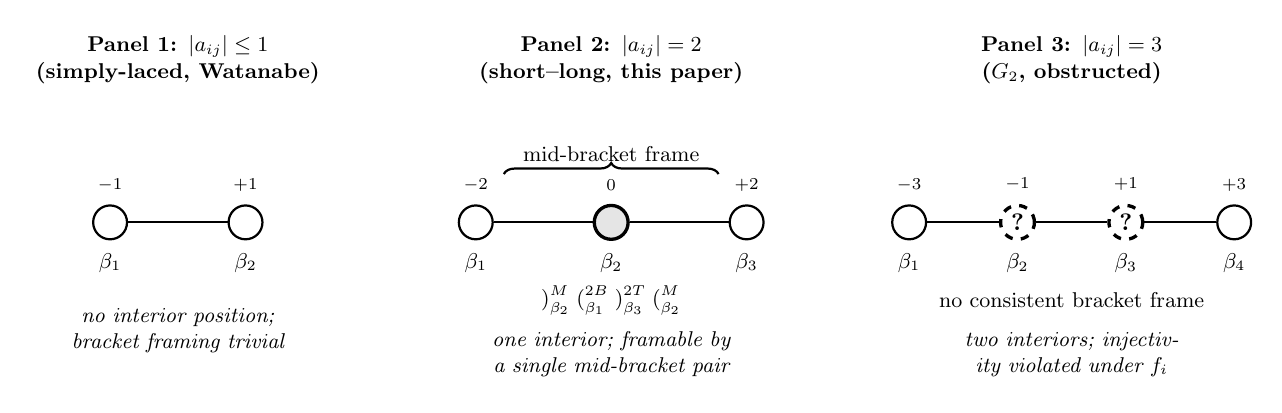
\begin{tikzpicture}[scale=0.86, transform shape,
  every node/.style={font=\small},
  chainnode/.style={circle, draw, thick, minimum size=5mm, inner sep=0pt, fill=white},
  interior/.style={circle, draw, very thick, minimum size=5mm, inner sep=0pt, fill=black!10},
  badinterior/.style={circle, draw, very thick, minimum size=5mm, inner sep=0pt, fill=white, dashed},
  bond/.style={thick},
  brace/.style={decorate, decoration={brace, amplitude=4pt, raise=4pt}, thick},
  panellabel/.style={font=\small\itshape, align=center, text width=4.2cm},
  paneltitle/.style={font=\small\bfseries, align=center}
]

%========== PANEL 1: simply-laced, |a| <= 1 ==========
\begin{scope}[xshift=0cm]
  \node[paneltitle] at (1.0, 2.6) {Panel 1: $|a_{ij}| \leq 1$};
  \node[paneltitle] at (1.0, 2.2) {(simply-laced, Watanabe)};

  \node[chainnode] (a1) at (0, 0) {};
  \node[chainnode] (a2) at (2, 0) {};
  \draw[bond] (a1) -- (a2);

  \node[below=2pt] at (a1.south) {$\beta_1$};
  \node[below=2pt] at (a2.south) {$\beta_2$};
  \node[above=2pt] at (a1.north) {\scriptsize $-1$};
  \node[above=2pt] at (a2.north) {\scriptsize $+1$};

  \node[panellabel] at (1.0, -1.6) {no interior position; bracket framing trivial};
\end{scope}

%========== PANEL 2: short-long, |a| = 2 (this paper) ==========
\begin{scope}[xshift=5.4cm]
  \node[paneltitle] at (2.0, 2.6) {Panel 2: $|a_{ij}| = 2$};
  \node[paneltitle] at (2.0, 2.2) {(short--long, \textbf{this paper})};

  \node[chainnode] (b1) at (0, 0) {};
  \node[interior]  (b2) at (2, 0) {};
  \node[chainnode] (b3) at (4, 0) {};
  \draw[bond] (b1) -- (b2) -- (b3);

  \node[below=2pt] at (b1.south) {$\beta_1$};
  \node[below=2pt] at (b2.south) {$\beta_2$};
  \node[below=2pt] at (b3.south) {$\beta_3$};
  \node[above=2pt] at (b1.north) {\scriptsize $-2$};
  \node[above=2pt] at (b2.north) {\scriptsize $0$};
  \node[above=2pt] at (b3.north) {\scriptsize $+2$};

  \draw[brace] ($(b1.east) + (0.15, 0.55)$) -- ($(b3.west) + (-0.15, 0.55)$)
    node[midway, above=6pt] {mid-bracket frame};

  \node[font=\small, align=center] at (2, -1.15)
    {$\labr{\beta_2}^{M}\;\labl{\beta_1}^{2B}\;\labr{\beta_3}^{2T}\;\labl{\beta_2}^{M}$};

  \node[panellabel] at (2.0, -1.95) {one interior; framable by a single mid-bracket pair};
\end{scope}

%========== PANEL 3: G_2, |a| = 3 ==========
\begin{scope}[xshift=11.8cm]
  \node[paneltitle] at (2.4, 2.6) {Panel 3: $|a_{ij}| = 3$};
  \node[paneltitle] at (2.4, 2.2) {($G_2$, obstructed)};

  \node[chainnode]   (c1) at (0, 0) {};
  \node[badinterior] (c2) at (1.6, 0) {};
  \node[badinterior] (c3) at (3.2, 0) {};
  \node[chainnode]   (c4) at (4.8, 0) {};
  \draw[bond] (c1) -- (c2) -- (c3) -- (c4);

  \node[below=2pt] at (c1.south) {$\beta_1$};
  \node[below=2pt] at (c2.south) {$\beta_2$};
  \node[below=2pt] at (c3.south) {$\beta_3$};
  \node[below=2pt] at (c4.south) {$\beta_4$};
  \node[above=2pt] at (c1.north) {\scriptsize $-3$};
  \node[above=2pt] at (c2.north) {\scriptsize $-1$};
  \node[above=2pt] at (c3.north) {\scriptsize $+1$};
  \node[above=2pt] at (c4.north) {\scriptsize $+3$};

  \node[font=\bfseries] at (c2.center) {?};
  \node[font=\bfseries] at (c3.center) {?};

  \node[font=\small, align=center] at (2.4, -1.15) {no consistent bracket frame};
  \node[panellabel] at (2.4, -1.95) {two interiors; injectivity violated under $f_i$};
\end{scope}

\end{tikzpicture}
\caption{The bracket framework for $\Cmid_a$ admits clean structure only at
$|a_{ij}| \leq 2$: simply-laced edges have no interior (left), the short--long edge has
exactly one interior framable by a single mid-bracket pair (centre, this paper), and the
$G_2$ triple edge has two interiors with no consistent framing (right). Numbers above each
chain node record the pairing $\langle \beta_k, \alpha_i^\vee\rangle$ with the active simple
coroot.}
\label{fig:bracket-trichotomy}
\end{figure}

%==============================================================================
\section{Preliminaries}\label{sec:prelim}
%==============================================================================

\subsection{Notation for type $B_n$}\label{ssec:notation-Bn}

Throughout, $\g$ is the complex simple Lie algebra of type $B_n$ for some $n \geq 2$. We
realise its root system in $\mathbb{R}^n$ with standard basis $E_1, \ldots, E_n$. The simple
roots are
\[
\alpha_a = E_a - E_{a+1} \quad (1 \leq a < n), \qquad \alpha_n = E_n.
\]
The roots $\alpha_1, \ldots, \alpha_{n-1}$ are \emph{long}; $\alpha_n$ is \emph{short}. The
positive roots are
\[
\Phi^+(B_n) \;=\; \{E_a : 1 \leq a \leq n\} \;\cup\; \{E_a - E_b, E_a + E_b : 1 \leq a < b \leq n\}.
\]
The Cartan matrix entries are $a_{a,a+1} = a_{a+1,a} = -1$ for $1 \leq a < n-1$, $a_{n-1,n} =
-2$, $a_{n,n-1} = -1$, and $a_{i,i} = 2$. The entry $a_{n-1,n} = -2$ is the \emph{short--long
edge} that fails $(\mathrm{S1})$--$(\mathrm{S3})'$ of \cite{Watanabe2110}.

We work over a field $\KK$ of characteristic zero throughout (typically $\KK = \mathbb{Q}(q)$
at generic $q$, specialising to $q = 0$ at the crystal limit).

\subsection{Kashiwara crystals and $\imath$-crystals}\label{ssec:kashiwara}

Kashiwara's crystal basis \cite{Kashiwara1991} attaches to each finite-type quantum group
$\Uq$ and each integrable highest-weight module a combinatorial datum $(B, \tilde e_i,
\tilde f_i, \varepsilon_i, \varphi_i, \mathrm{wt})$ obtained as the $q = 0$ limit of a
canonical basis. The lowest-weight crystal $B(\infty)$ of $\Uqm$ admits an explicit realisation
on Kostant partitions:
\[
\Kp(\infty) \;:=\; \bigoplus_{\pi \in \Zn^{\Phi^+}} \KK \cdot \pi,
\]
where each $\pi = (c_\beta)_{\beta \in \Phi^+}$ is a vector of nonnegative root multiplicities
and the Kashiwara operators $\tilde e_i, \tilde f_i$ are computed by the bracketing procedure
recalled in Section~\ref{ssec:bracket-alphabet}.

\medskip
\noindent\textbf{The $\imath$-crystal extension.}
For a quantum symmetric pair $(\Uq, \Uiota)$ of finite type, the $\imath$-coideal subalgebra
$\Uiota$ is generated by symbols $B_i = F_i + \varsigma_n T_i(\Theta)$ that twist the Chevalley
$F_i$ by Kashiwara--Lusztig-style adjoint terms. At $q = 0$, $B_i$ specialises to a
single combinatorial operator on $\Kp(\infty)$ which Watanabe \cite{Watanabe2107} writes as
\[
B_i \;=\; \tilde e_i + \tilde f_i \quad (\text{at } q = 0)
\]
when the node $i$ is split, i.e., $a_{i,\tau(i)} = 2$. (Other cases of $a_{i,\tau(i)} \in
\{0, -1\}$ give different combinatorial operators; see \cite[\S4.1]{Watanabe2110}.) The pair
$(\Kp(\infty), B_i)$ for $i$ ranging over the Satake diagram is the \emph{$\imath$-crystal}
of $\Uiota$ at the chosen quantum symmetric pair.

For type BDI, $\tau = \mathrm{id}$, so every node is split and $a_{i,\tau(i)} = 2$ for all $i$.
The combinatorial operator $B_i = \tilde e_i + \tilde f_i$ acts on $\Kp(\infty)$ for each
simple root $\alpha_i$. The present paper studies the case $i = n$, the short simple.

\begin{remark}[Parameter convention for $\varsigma_n$]\label{rmk:varsigma-convention}
Following Watanabe \cite[\S3.3(D)]{Watanabe2110}, the parameter $\varsigma_n$ lies in
$\{q_n^a : a \in \mathbb{Z}\}$; the main theorem is independent of the choice of
$\varsigma_n$ in this set, so we normalise $\varsigma_n = 1$ in computations.
\end{remark}

\subsection{The bracket alphabet}\label{ssec:bracket-alphabet}

The Kashiwara operators are computed via a bracket-sequence procedure that we now recall in
the form used throughout the paper. This is the CST formulation of \cite[Definition~2.14]{CST}
(see also Salisbury--Tingley); we extend the standard signature to handle the doubled
contribution at $a_{ij} = -2$.

\medskip
\noindent\textbf{Symbols.}
The bracket alphabet consists of two symbols, $\labl{}$ (raising) and $\labr{}$ (lowering),
each carrying a label in $\Phi^+$. Concatenations of bracket symbols form bracket sequences.
The number of symbols an individual root $\beta$ contributes is governed by its pairing with
the simple coroot $\alpha_i^\vee$ at which we read brackets:
\[
\#\text{ of }\labr{\beta}\text{s contributed per multiplicity of }\beta \;=\; \max(0,\;\langle
\beta, \alpha_i^\vee\rangle), \qquad
\#\text{ of }\labl{\beta}\text{s} \;=\; \max(0,\;-\langle \beta, \alpha_i^\vee\rangle).
\]
For the short simple of $B_n$, the pairings are $\langle E_a - E_n, \alpha_n^\vee\rangle =
-2$, $\langle E_a, \alpha_n^\vee\rangle = 0$, $\langle E_a + E_n, \alpha_n^\vee\rangle = +2$,
and $\langle E_n, \alpha_n^\vee\rangle = +2$. The middle case requires care: the root $E_a$
with $\langle E_a, \alpha_n^\vee\rangle = 0$ contributes both raising and lowering symbols
because it has nonzero $\alpha_n$-string length, namely both $E_a + E_n$ and $E_a - E_n$ are
in $\Phi^+$. The standard convention (see \cite[\S2]{Kashiwara1991}) places one $\labr{E_a}$
per multiplicity \emph{before} the contributions of $E_a + E_n, E_a - E_n$ and one
$\labl{E_a}$ \emph{after}.

\medskip
\noindent\textbf{Cancellation.}
The bracket sequence is canonicalised by repeated cancellation: any adjacent pair $\labl{}
\labr{}$ (a raising symbol immediately followed by a lowering symbol) is removed. The
process terminates and produces a canonical sequence with all surviving $\labr{}$s to the
left of all surviving $\labl{}$s. The cancellation respects bracket labels in the sense that
the labels do not affect which symbols cancel, only what label appears on the resulting
operator.

\medskip
\noindent\textbf{Operators from brackets.}
Given the canonical bracket sequence of $\pi$ at the simple root $\alpha_i$:
\begin{itemize}[leftmargin=2em]
  \item $\varepsilon_i(\pi)$ is the number of surviving $\labr{}$s.
  \item $\varphi_i(\pi)$ is the number of surviving $\labl{}$s.
  \item $\tilde e_i(\pi)$ acts on the rightmost surviving $\labr{}$, with label $\beta$; the
    action on $\pi$ is $\pi \mapsto \pi - e_\beta + e_{\beta - \alpha_i}$ when $\beta \neq
    \alpha_i$, and $\pi \mapsto \pi - e_{\alpha_i}$ when $\beta = \alpha_i$.
  \item $\tilde f_i(\pi)$ acts on the leftmost surviving $\labl{}$ symmetrically.
\end{itemize}

\medskip
\noindent\textbf{Extension at $a_{ij} = -2$.}
The convention above gives the doubled exponents naturally: the root $E_a + E_n$, having
$\langle \cdot, \alpha_n^\vee\rangle = 2$, contributes $\labr{E_a + E_n}^2$ per multiplicity,
and similarly $E_a - E_n$ contributes $\labl{E_a - E_n}^2$ per multiplicity. These doubled
symbol counts are the bracket-level expression of the short--long Cartan entry $|a_{n,a}|
= 2$.

\subsection{The slice $K_p(\infty)$ and step types}\label{ssec:slice}

For the rest of the paper we fix the short simple $i = n$ and abbreviate $\varepsilon =
\varepsilon_n$, $\varphi = \varphi_n$, $\tilde e = \tilde e_n$, $\tilde f = \tilde f_n$, and
write $B := B_n = \tilde e + \tilde f$ for the $\imath$-coideal generator at the short node.

\begin{definition}\label{def:slice}
The \emph{depth-$k$ slice} of $\Kp(\infty)$ at the short simple is
\[
S_n^{(k)} \;:=\; \{\pi \in \Kp(\infty) : \varepsilon(\pi) \geq k\}.
\]
For $k = 2$ we abbreviate $S_n := S_n^{(2)}$ and call it simply the \emph{slice} (or
\emph{on-slice} part) when the value of $k$ is clear from context.
\end{definition}

The combinatorial object of central interest is the multiset of net deltas of $\tilde e^2$
on the slice:
\[
C_n \;:=\; \bigl\{\,\tilde e^2(\pi) - \pi \;:\; \pi \in S_n\,\bigr\},
\]
called the \emph{$e_n^2$ catalog}. The size of this catalog and its structural decomposition
into three classes are the empirical content that the tensor product rule will explain.

\medskip
\noindent\textbf{$\alpha_n$-orbits on $\Phi^+$.}
The action of the short reflection $s_n$ partitions $\Phi^+(B_n)$ into three families:

\begin{itemize}[leftmargin=2em]
  \item \emph{Chains.} For each $a \in \{1, \ldots, n-1\}$,
    \[
    \Chain(a) \;=\; \{E_a - E_n,\; E_a,\; E_a + E_n\}
    \]
    is a length-three $\alpha_n$-string with $E_a$ as the middle root.
  \item \emph{Singleton.} $\Sing = \{E_n\}$, a length-one $\alpha_n$-string. ($\alpha_n$
    itself.)
  \item \emph{Non-touching.} $\NT = \{E_a \pm E_b : 1 \leq a < b < n\}$, length-one
    $\alpha_n$-strings with $\langle \cdot, \alpha_n^\vee\rangle = 0$ and with no neighbouring
    root in $\Phi^+ \cup \{0\}$ across $\pm \alpha_n$.
\end{itemize}

The non-touching roots contribute no bracket symbols at $\alpha_n$ (raising and lowering
counts both zero) and so play no role in the $B_n$-action. We omit them from the tensor
product decomposition; see Remark~\ref{rmk:non-touching} for the bookkeeping needed if one
wishes to include them as trivial factors.

\subsection{Step types}\label{ssec:step-types}

\begin{definition}\label{def:step-types}
The \emph{step types} of $\tilde e$ on $\Kp(\infty)|_{B_n}$ are the labelled actions on
$\pi$ that arise from acting on a rightmost surviving $\labr{}$ at the short simple. They are:
\begin{align*}
\MB(a) &: \quad \pi \mapsto \pi - e_{E_a} + e_{E_a - E_n}, \quad a \in \{1, \ldots, n-1\}, \\
\TM(a) &: \quad \pi \mapsto \pi - e_{E_a + E_n} + e_{E_a}, \quad a \in \{1, \ldots, n-1\}, \\
\Sing &: \quad \pi \mapsto \pi - e_{E_n}.
\end{align*}
\end{definition}

The labels MB and TM are mnemonics: MB ``mid drops to bot'' and TM ``top drops to mid'' along
the chain. There are $2(n-1) + 1 = 2n - 1$ step types in total.

\subsection{The chain factor and singleton factor}\label{ssec:factors}

We now define the two building blocks of the tensor product decomposition.

\begin{definition}[Chain factor]\label{def:chain-factor}
For each $a \in \{1, \ldots, n-1\}$, the \emph{chain factor} is the $\Zn^3$-graded vector space
\[
\Cmid_a \;:=\; \KK\bigl\langle (M, B, T) : M, B, T \in \Zn \bigr\rangle
\]
on three generators of grades $E_a$ (\emph{mid}), $E_a - E_n$ (\emph{bot}), $E_a + E_n$
(\emph{top}). Its \emph{internal bracket block} at the short simple $\alpha_n$ is the bracket
sequence
\begin{equation}\label{eq:chain-bracket-block}
\br(\Cmid_a)(M, B, T) \;=\; \labr{E_a}^{M}\;\labl{E_a - E_n}^{2B}\;\labr{E_a + E_n}^{2T}\;\labl{E_a}^{M}.
\end{equation}
\end{definition}

\begin{definition}[Singleton factor]\label{def:singleton-factor}
The \emph{singleton factor} is the $\Zn$-graded vector space
\[
\Csing \;:=\; \KK[B_n] \;\cong\; \bigoplus_{S \geq 0} \KK \cdot B_n^S,
\]
i.e., the polynomial algebra on the generator $B_n$ itself. Its internal bracket block at
the short simple is
\begin{equation}\label{eq:sing-bracket-block}
\br(\Csing)(S) \;=\; \labr{E_n}^{S}.
\end{equation}
\end{definition}

\begin{remark}[Doubling and the short--long edge]\label{rmk:doubling}
The doubled exponents $2B$ and $2T$ in (\ref{eq:chain-bracket-block}) are the bracket-level
realisation of the off-diagonal Cartan entries
\[
\langle E_a - E_n, \alpha_n^\vee\rangle \;=\; -2, \qquad \langle E_a + E_n, \alpha_n^\vee\rangle \;=\; +2,
\]
equivalent to $|a_{n,a}| = 2$ for the short--long edge. The mid-framing $\labr{E_a}^M \cdots
\labl{E_a}^M$ is the bracket-level expression of $\langle E_a, \alpha_n^\vee\rangle = 0$
combined with the fact that $E_a$ has a non-trivial $\alpha_n$-string of length three; the
mid root contributes both raising and lowering symbols, with the bot- and top-contributions
sandwiched between them.
\end{remark}

\begin{remark}[Comparison with Watanabe]\label{rmk:watanabe-vs-chain}
The singleton factor $\Csing$ is exactly Watanabe's split-node rank-one $\imath$-crystal
$U^n_n = \KK[B_n]$ from \cite[\S4.1]{Watanabe2110} at the split node $a_{n,\tau(n)} = 2$.
The chain factor $\Cmid_a$ has no counterpart in \cite{Watanabe2110}: the framework there has
only rank-one per-node objects glued by simply-laced edges, and the short--long edge $a_{n-1,n}
= -2$ requires the new rank-three building block $\Cmid_a$ to encode the doubled bracket
contribution.
\end{remark}

%==============================================================================
\section{Main theorem and Phase A}\label{sec:main}
%==============================================================================

\subsection{Statement of the main theorem}

\begin{theorem}[Main theorem]\label{thm:main}
Let $\g$ be of type $B_n$, $n \geq 2$, and let $B_n = F_n + \varsigma_n E_n K_n^{-1}$ be the
short-simple $\imath$-coideal generator. There is an isomorphism of $\imath$-crystals
\begin{equation}\label{eq:main}
\Kp(\infty)\big|_{B_n} \;\cong\; \bigotimes_{a=1}^{n-1} \Cmid_a \;\otimes\; \Csing,
\end{equation}
where $\Cmid_a$ is the chain factor of Definition~\ref{def:chain-factor} and $\Csing$ is the
singleton factor of Definition~\ref{def:singleton-factor}. The isomorphism sends
\[
\bigl((M_a, B_a, T_a)_{a=1}^{n-1},\; S\bigr) \;\longmapsto\;
\sum_{a=1}^{n-1} \bigl(M_a\, E_a + B_a\, (E_a - E_n) + T_a\, (E_a + E_n)\bigr) + S\, E_n,
\]
and intertwines the tensor-product bracket of the right-hand side (concatenation in convex
chain order followed by the singleton block, with cancellation propagating across factor
boundaries) with the standard short-simple bracket sequence of $\Kp(\infty)$.

The $e_n^2$ catalog on the slice $S_n$ has size $\binom{2n}{2} = n(2n - 1)$, decomposing as
\begin{equation}\label{eq:catalog-count}
n(2n - 1) \;=\; \underbrace{3(n-1)}_{\textnormal{intra-chain}} \;+\;
\underbrace{2(n-1)(n-2)}_{\textnormal{cross-chain}} \;+\;
\underbrace{(2n-1)}_{\textnormal{singleton-involving}},
\end{equation}
where the three classes correspond to the three possible factor incidences of an unordered
pair of step-type primitives: both in a common $\Cmid_a$ (intra-chain), in distinct $\Cmid_a
\neq \Cmid_b$ (cross-chain), or at least one in $\Csing$ (singleton-involving).
\end{theorem}

\begin{corollary}\label{cor:catalog}
The counts $n(2n-1) = 3(n-1) + 2(n-1)(n-2) + (2n-1)$ match the empirically observed catalog
sizes at $B_2$ (6 entries), $B_3$ (15), $B_4$ (28), $B_5$ (45), with the three-class split
$3 + 0 + 3$, $6 + 4 + 5$, $9 + 12 + 7$, $12 + 24 + 9$ respectively.
\end{corollary}

\begin{remark}[Non-touching factors]\label{rmk:non-touching}
The isomorphism (\ref{eq:main}) is between the right-hand side and the chain-plus-singleton
sector of $\Kp(\infty)|_{B_n}$. The non-touching roots $\NT$ of Section~\ref{ssec:slice}
contribute $\binom{n-1}{2} + \binom{n-1}{2} = (n-1)(n-2)$ trivial factors, each a one-dimensional
$\imath$-crystal under $B_n$-action ($\tilde e_n = \tilde f_n = 0$, $\varepsilon = \varphi
= 0$). Adjoining these factors changes neither the bracket structure nor the $e_n^2$ catalog,
so we omit them for clarity. (They are relevant only when the long-simple operators $B_a$ are
brought back into the picture, which is outside the scope of this paper.)
\end{remark}

The proof of Theorem~\ref{thm:main} is given in four phases. Phase A is proved in
Section~\ref{ssec:phaseA} below; Phases B--D occupy Sections \ref{sec:phaseB}--\ref{sec:phaseD}.

\subsection{Phase A: chain factor uniformity}\label{ssec:phaseA}

Phase A asserts that the chain factor $\Cmid_a$ is structurally the same for every $a$ and
every $n$, with only the labels on bracket symbols varying with $a$.

\begin{lemma}[Phase A: structural uniformity of chain factors]\label{lem:phaseA}
For all $a, a' \in \{1, \ldots, n-1\}$ and all $n \geq 2$:
\begin{itemize}[leftmargin=2em]
  \item[(i)] $\Cmid_a$ and $\Cmid_{a'}$ are isomorphic as graded vector spaces (both are
    polynomial rings in three generators, with no $a$-dependence in the grading lattice up to
    relabelling).
  \item[(ii)] The internal bracket blocks $\br(\Cmid_a)$ and $\br(\Cmid_{a'})$ have identical
    shape: four sub-blocks of widths $M, 2B, 2T, M$ with bracket types $\labr{}, \labl{},
    \labr{}, \labl{}$ in that order, differing only in the labels attached to the bracket
    symbols (where $E_a$ is replaced by $E_{a'}$ and $E_a \pm E_n$ by $E_{a'} \pm E_n$).
\end{itemize}
\end{lemma}

\begin{proof}
Part (i) is immediate: $\Cmid_a$ is the polynomial ring on three generators of grades
$(\mathrm{mid}_a, \mathrm{bot}_a, \mathrm{top}_a) = (E_a, E_a - E_n, E_a + E_n)$, with grading
lattice $\Z \cdot E_a \oplus \Z \cdot (E_a - E_n) \oplus \Z \cdot (E_a + E_n) \cong \Z^3$ via
the obvious basis. The lattice is independent of $a$ up to relabelling.

Part (ii) is the content of the lemma. The internal bracket block (\ref{eq:chain-bracket-block})
is determined by two pieces of data:
\begin{itemize}[leftmargin=2em]
  \item the \emph{local pairings} of $\alpha_n^\vee$ with the three chain roots, namely
    \[
    \langle E_a - E_n, \alpha_n^\vee\rangle = -2, \qquad \langle E_a, \alpha_n^\vee\rangle = 0, \qquad \langle E_a + E_n, \alpha_n^\vee\rangle = +2;
    \]
  \item the \emph{chain position} of each root (top, mid, or bot) within the length-three
    $\alpha_n$-string $\Chain(a)$.
\end{itemize}
Both pieces of data depend only on the \emph{type} of the root (long $E_a \pm E_n$ versus
short $E_a$) and its $\alpha_n^\vee$-pairing, not on the index $a$. The bracket-alphabet
rule of Section~\ref{ssec:bracket-alphabet} translates these uniformly:
\begin{itemize}[leftmargin=2em]
  \item Top, with $\langle \cdot, \alpha_n^\vee\rangle = +2$, contributes $\labr{}^{2T}$ per
    multiplicity $T$.
  \item Bot, with $\langle \cdot, \alpha_n^\vee\rangle = -2$, contributes $\labl{}^{2B}$ per
    multiplicity $B$.
  \item Mid, with $\langle \cdot, \alpha_n^\vee\rangle = 0$ but with non-trivial $\alpha_n$-
    string of length three, contributes both $\labr{}^M$ (leading) and $\labl{}^M$ (trailing)
    per multiplicity $M$, with the bot- and top-contributions sandwiched between them.
\end{itemize}
The resulting block shape $\labr{}^M\, \labl{}^{2B}\, \labr{}^{2T}\, \labl{}^M$ is therefore
the same for every $a$, with only the labels relabelled $E_a \to E_{a'}$, $E_a \pm E_n \to
E_{a'} \pm E_n$.
\end{proof}

\begin{remark}[Mid-framing comes from $\langle \mathrm{mid}, \alpha_n^\vee\rangle = 0$]\label{rmk:mid-framing}
The mid framing $\labr{E_a}^M \cdots \labl{E_a}^M$ surrounding the bot- and top-contributions
is the bracket-level encoding of the fact that the chain middle is \emph{fixed} by the short
reflection $s_n$ while still belonging to an $\alpha_n$-string of length three (its neighbours
$E_a \pm E_n$ are positive roots). The mid contributes both raising and lowering capacity per
multiplicity --- $\labr{E_a}$s for $\tilde e_n$ and $\labl{E_a}$s for $\tilde f_n$ --- but at
different positions in the bracket order, with the leading $\labr{E_a}$s bracket-precedent and
the trailing $\labl{E_a}$s bracket-subsequent.
\end{remark}

\begin{remark}[Doubling is exactly $a_{n,a} = -2$]\label{rmk:doubling-detail}
The factor of $2$ in the exponents $2B$ and $2T$ is the bracket-level expression of the
short--long Cartan entry $|a_{n,a}| = 2$ (equivalently, $\langle E_a \pm E_n, \alpha_n^\vee
\rangle = \pm 2$). The framework of \cite{Watanabe2110} handles only $|a_{ij}| \leq 1$ via
$(\mathrm{S1})$--$(\mathrm{S3})'$. The doubled bracket block is the new ingredient introduced
by the present paper.
\end{remark}

%==============================================================================
\section{Phase B: tensor product as $\imath$-crystal}\label{sec:phaseB}
%==============================================================================

Phase A has produced the building blocks. Phase B assembles them into a tensor
product carrying an $\imath$-crystal structure and identifies that tensor product
with $\Kp(\infty)|_{B_n}$ on the nose. The identification is tautological: the
tensor-product bracket of $\bigotimes_a \Cmid_a \otimes \Csing$ is literally the
CST bracketing of $\Kp(\infty)$ read as a string concatenation, provided the
factor blocks are arranged in convex chain order.

\subsection{The tensor product as a graded vector space}\label{ssec:tensor-graded}

\begin{definition}[Tensor product factor and its bracket]\label{def:tensor-bracket}
For $n \geq 2$, the \emph{chain-plus-singleton tensor product} is
\[
\TT_n \;:=\; \bigotimes_{a=1}^{n-1} \Cmid_a \;\otimes\; \Csing,
\]
a $\Zn^{3(n-1) + 1}$-graded vector space with basis
$\bigl((M_a, B_a, T_a)_{a=1}^{n-1},\, S\bigr)$, where $(M_a, B_a, T_a) \in \Zn^3$
is the multidegree in $\Cmid_a$ and $S \in \Zn$ is the multidegree in $\Csing$.
Its \emph{tensor-product bracket} at the short simple $\alpha_n$ is the string
concatenation
\begin{equation}\label{eq:tensor-bracket}
\br_{\TT_n}\bigl((M_a, B_a, T_a)_a,\, S\bigr) \;=\;
\br(\Cmid_1)(M_1, B_1, T_1) \cdot \br(\Cmid_2)(M_2, B_2, T_2) \cdots \br(\Cmid_{n-1})(M_{n-1}, B_{n-1}, T_{n-1}) \cdot \br(\Csing)(S),
\end{equation}
i.e., the chain blocks in increasing-$a$ (convex) order followed by the singleton
block. Cancellation is then applied to the full concatenated string by the rule of
Section~\ref{ssec:bracket-alphabet}: adjacent $\labl{}\labr{}$ pairs are deleted
repeatedly, \emph{across factor boundaries}, until the canonical form is reached.
\end{definition}

\begin{definition}[$\imath$-crystal operators on $\TT_n$]\label{def:tensor-icrystal-ops}
The operators $\tilde e_n, \tilde f_n$ act on $\TT_n$ by the bracket procedure of
Section~\ref{ssec:bracket-alphabet} applied to (\ref{eq:tensor-bracket}):
\begin{itemize}[leftmargin=2em]
  \item $\varepsilon_n$ is the number of surviving $\labr{}$s after cancellation.
  \item $\varphi_n$ is the number of surviving $\labl{}$s.
  \item $\tilde e_n$ acts on the rightmost surviving $\labr{}$, with label $\beta$,
    by updating the multiplicity in the factor whose block contributed that symbol:
    decrement $e_\beta$ and increment $e_{\beta - \alpha_n}$ in that factor (or
    decrement $e_{\alpha_n}$ if $\beta = \alpha_n$).
  \item $\tilde f_n$ acts on the leftmost surviving $\labl{}$ symmetrically.
\end{itemize}
The $\imath$-coideal generator at $q = 0$ is $B_n = \tilde e_n + \tilde f_n$, as in
Section~\ref{ssec:kashiwara}.
\end{definition}

\subsection{Identification with $\Kp(\infty)|_{B_n}$}\label{ssec:tensor-identification}

\begin{theorem}[Tensor product equals CST bracketing]\label{thm:phaseB-identification}
The map
\begin{equation}\label{eq:phaseB-iota}
\iota:\ \TT_n \;\longrightarrow\; \Kp(\infty)\big|_{B_n},
\quad
\bigl((M_a, B_a, T_a)_{a=1}^{n-1},\, S\bigr) \;\longmapsto\;
\sum_{a=1}^{n-1} \bigl(M_a\, E_a + B_a\, (E_a - E_n) + T_a\, (E_a + E_n)\bigr) + S\, E_n
\end{equation}
is an isomorphism onto the chain-plus-singleton sector of $\Kp(\infty)$ as a
graded vector space, and intertwines the tensor-product bracket $\br_{\TT_n}$ of
Definition~\ref{def:tensor-bracket} with the standard short-simple CST bracket
sequence of $\Kp(\infty)$. Hence $\iota$ intertwines the operators $\tilde e_n,
\tilde f_n$ and $B_n$ on both sides, and $\TT_n$ inherits the $\imath$-crystal
structure of $\Kp(\infty)|_{B_n}$ on the chain-plus-singleton sector.
\end{theorem}

\begin{proof}
\emph{Graded vector space.} The map $\iota$ sends the tensor-product basis element
$\bigl((M_a, B_a, T_a)_a, S\bigr)$ to the Kostant partition with multiplicities
$M_a$ on $E_a$, $B_a$ on $E_a - E_n$, $T_a$ on $E_a + E_n$, and $S$ on $E_n$, and
zero on all other positive roots. This is a bijection onto the sublattice of
$\Kp(\infty)$ supported on $\bigcup_a \Chain(a) \cup \Sing$. The remaining roots,
the non-touching family $\NT$, form a disjoint complementary sublattice;
see Remark~\ref{rmk:non-touching}.

\emph{Bracket intertwining.} The CST bracketing of $\pi = \iota\bigl((M_a, B_a, T_a)_a,\, S\bigr)$
at the short simple, read off according to Section~\ref{ssec:bracket-alphabet}, is
\begin{equation}\label{eq:CST-bracket-Kp}
\br_{\Kp(\infty)}(\pi) \;=\;
\bigl[\,\labr{E_a}^{M_a}\, \labl{E_a - E_n}^{2B_a}\, \labr{E_a + E_n}^{2T_a}\, \labl{E_a}^{M_a}\,\bigr]_{a=1}^{n-1}\,
\labr{E_n}^{S},
\end{equation}
where the blocks are arranged in convex order of the mid root $E_a$
(chain $1$, then chain $2$, $\ldots$, then chain $n-1$), and the singleton
block $\labr{E_n}^S$ is appended last. The bracket symbols contributed by the
non-touching roots in $\NT$ are absent: each has $\langle \cdot, \alpha_n^\vee\rangle = 0$
and a trivial $\alpha_n$-string, so the rule of Section~\ref{ssec:bracket-alphabet}
contributes neither $\labr{}$s nor $\labl{}$s.

Comparing (\ref{eq:CST-bracket-Kp}) with (\ref{eq:tensor-bracket}) and the
per-factor bracket blocks (\ref{eq:chain-bracket-block}) and
(\ref{eq:sing-bracket-block}), the two expressions are character-for-character
identical with the substitutions $(M_a, B_a, T_a, S) = (c_{E_a}, c_{E_a - E_n},
c_{E_a + E_n}, c_{E_n})$. The cancellation rule is also identical on both sides:
adjacent $\labl{}\labr{}$ pairs are deleted regardless of label, and the
cancellation is global (across factor boundaries) on $\TT_n$ by
Definition~\ref{def:tensor-bracket} and global by construction on $\Kp(\infty)$.

\emph{Operator intertwining.} Since the bracket sequences and their canonical
forms agree, the surviving $\labr{}$ and $\labl{}$ symbols are in canonical
bijection, with matching labels. Acting on the rightmost surviving $\labr{}$ on
$\TT_n$ updates the multiplicity in the factor whose block contributed it; under
$\iota$, the same update is applied to the corresponding root in $\Kp(\infty)$.
Hence $\iota$ intertwines $\tilde e_n$, and symmetrically $\tilde f_n$ and
$B_n = \tilde e_n + \tilde f_n$.
\end{proof}

\begin{remark}[$\imath$-crystal axioms]\label{rmk:icrystal-axioms}
The $\imath$-crystal axioms (compatibility of $\varepsilon_n, \varphi_n,
\tilde e_n, \tilde f_n$ with the weight grading; Kashiwara's signature rule)
hold on $\TT_n$ tautologically: $\TT_n$ is isomorphic via $\iota$ to the
chain-plus-singleton sector of $\Kp(\infty)$, which inherits its $\imath$-crystal
structure from the Kashiwara crystal of $\Uqm$. The substantive content of
Definition~\ref{def:tensor-bracket} is not that $\TT_n$ is an $\imath$-crystal
--- that follows from Theorem~\ref{thm:phaseB-identification} --- but that the
$\imath$-crystal structure \emph{factorises} as a tensor product of chain factors
and a singleton factor, with the explicit concatenation-of-bracket-blocks rule.
This factorisation is the content beyond \cite[Prop.~5.1.1]{Watanabe2110}: the
latter provides such a factorisation only for simply-laced edges
$a_{ij} \in \{0, -1\}$ satisfying $(\mathrm{S1})$--$(\mathrm{S3})'$.
\end{remark}

\begin{lemma}[Per-node match for the singleton factor]\label{lem:singleton-watanabe-match}
The singleton factor $\Csing = \KK[B_n]$ of Definition~\ref{def:singleton-factor},
equipped with the $\imath$-crystal operators of
Definition~\ref{def:tensor-icrystal-ops}, coincides with Watanabe's split-node
rank-one $\imath$-crystal $U^n_n = \KK[B_n]$ of \cite[\S4.1]{Watanabe2110} at
$a_{n,\tau(n)} = 2$.
\end{lemma}

\begin{proof}
Both objects have underlying vector space $\KK[B_n] = \bigoplus_{S \geq 0} \KK\,B_n^S$
with single generator $B_n$. The bracket of $B_n^S$ at the short simple is
$\labr{E_n}^S$ by (\ref{eq:sing-bracket-block}); hence $\varepsilon_n(B_n^S) = S$,
$\varphi_n(B_n^S) = 0$, $\tilde e_n: B_n^S \mapsto B_n^{S-1}$, and
$\tilde f_n: B_n^S \mapsto B_n^{S+1}$. These match Watanabe's split-node rule
\cite[\S4.1, Case~$a_{i,\tau(i)} = 2$]{Watanabe2110}, in which the $\imath$-coideal
generator at a split node acts as $B_n: B_n^S \mapsto B_n^{S-1} + B_n^{S+1}$ at
$q = 0$, i.e., $B_n = \tilde e_n + \tilde f_n$.
\end{proof}

\begin{remark}[Chain factor as new building block]\label{rmk:chain-factor-new}
By contrast, the chain factor $\Cmid_a$ has no counterpart in
\cite[\S4.1]{Watanabe2110}: the per-node objects there are all of rank one, glued
across simply-laced edges by the tensor product rule of \cite[Prop.~5.1.1]{Watanabe2110}.
The doubled bracket exponents $2B$ and $2T$ in (\ref{eq:chain-bracket-block}) are
the bracket-level expression of the short--long Cartan entry $|a_{n-1, n}| = 2$,
which is excluded from $(\mathrm{S1})$--$(\mathrm{S3})'$. The rank-three building
block $\Cmid_a$ bundles together the three roots in $\Chain(a)$ and encodes the
short--long edge through its internal bracket block. The tensor product
$\bigotimes_a \Cmid_a \otimes \Csing$ thus extends Watanabe's framework across
the unique edge that was previously inaccessible.
\end{remark}

\begin{remark}[Non-touching factors, briefly]\label{rmk:non-touching-phaseB}
As noted in Remark~\ref{rmk:non-touching}, the non-touching roots $\NT$ contribute
$(n-1)(n-2)$ trivial factors to $\Kp(\infty)|_{B_n}$, each a one-dimensional
$\imath$-crystal with $\tilde e_n = \tilde f_n = 0$. Adjoining these factors to
$\TT_n$ replaces (\ref{eq:phaseB-iota}) by a bijection onto all of $\Kp(\infty)$
without changing the bracket structure or the operators $\tilde e_n, \tilde f_n,
B_n$ at the short simple. We work with $\TT_n$ as defined throughout the rest of
the paper; the non-touching factors re-enter the picture only under the
long-simple operators $B_a$ for $a < n$, which lie outside the present scope.
\end{remark}

%==============================================================================
\section{Phase C: on-slice catalog factor-by-factor}\label{sec:phaseC}
%==============================================================================

Phase C is the substantive combinatorial step. Each of the $\binom{2n}{2}$ entries
of the $e_n^2$ catalog $C_n$ is realised by an explicit Kostant-partition witness
whose support lies in at most two tensor factors of $\TT_n$. The witnesses are
type-uniform in the chain indices, and the bracket-level argument is the same for
adjacent and non-adjacent chain pairs because intermediate chains contribute no
bracket symbols when given zero multiplicity.

\subsection{Step types and factor incidence}\label{ssec:step-incidence}

Recall the step types of Definition~\ref{def:step-types}: the $2n - 1$ primitive
actions
\[
\{\MB(a) : 1 \leq a \leq n - 1\} \;\cup\; \{\TM(a) : 1 \leq a \leq n - 1\} \;\cup\; \{\Sing\},
\]
with net deltas $\delta_{\MB(a)} = -e_{E_a} + e_{E_a - E_n}$, $\delta_{\TM(a)} =
-e_{E_a + E_n} + e_{E_a}$, $\delta_{\Sing} = -e_{E_n}$. In the tensor-product
framing of Phase B, each step type corresponds to a primitive operator on a single
factor:

\begin{itemize}[leftmargin=2em]
  \item $\MB(a)$ and $\TM(a)$ are the two per-factor primitives on $\Cmid_a$: the
    chain-isolated action of $\tilde e_n$ on a state $(M, B, T) \in \Cmid_a$
    decrements $T$ and increments $M$ when $T > B$ (this is $\TM(a)$), or
    decrements $M$ and increments $B$ when $T \leq B$ and $M > 0$ (this is
    $\MB(a)$).
  \item $\Sing$ is the per-factor primitive on $\Csing$: decrement $S$.
\end{itemize}

\begin{definition}[Factor incidence]\label{def:factor-incidence}
Define $\mathrm{fac}(\MB(a)) = \mathrm{fac}(\TM(a)) = \Cmid_a$ and
$\mathrm{fac}(\Sing) = \Csing$. The \emph{factor incidence} of an unordered pair
(with repetition) $\{p, q\}$ of step types is the multiset
$\{\mathrm{fac}(p), \mathrm{fac}(q)\}$ of factors. The three structural classes
are:
\begin{itemize}[leftmargin=2em]
  \item \emph{Intra-chain}: $\mathrm{fac}(p) = \mathrm{fac}(q) = \Cmid_a$ for
    some $a$;
  \item \emph{Cross-chain}: $\mathrm{fac}(p) = \Cmid_a \neq \Cmid_b = \mathrm{fac}(q)$
    for some $a \neq b$, both chains;
  \item \emph{Singleton-involving}: at least one of $\mathrm{fac}(p), \mathrm{fac}(q)$
    equals $\Csing$.
\end{itemize}
\end{definition}

\begin{lemma}[Class counts]\label{lem:class-counts}
The number of unordered pairs (with repetition) of step types in each class is
\[
\#\textnormal{intra-chain} = 3(n-1),
\qquad
\#\textnormal{cross-chain} = 2(n-1)(n-2),
\qquad
\#\textnormal{singleton-involving} = 2n - 1.
\]
Their sum is $\binom{2n}{2} = n(2n - 1)$.
\end{lemma}

\begin{proof}
\emph{Intra-chain.} For each chain $a \in \{1, \ldots, n-1\}$, the unordered pairs
of primitives in $\Cmid_a$ are $\{\MB(a), \MB(a)\}$, $\{\TM(a), \TM(a)\}$, and
$\{\MB(a), \TM(a)\}$: three pairs per chain, $3(n-1)$ total.

\emph{Cross-chain.} For each unordered pair $\{a, b\}$ with $a \neq b$ in
$\{1, \ldots, n-1\}$, the four unordered pairs of primitives are $\{\MB(a),
\MB(b)\}$, $\{\MB(a), \TM(b)\}$, $\{\TM(a), \MB(b)\}$, $\{\TM(a), \TM(b)\}$: four
pairs per chain pair, $4\binom{n-1}{2} = 2(n-1)(n-2)$ total.

\emph{Singleton-involving.} The pair $\{\Sing, \Sing\}$ contributes one; the
pairs $\{\Sing, \MB(a)\}$ and $\{\Sing, \TM(a)\}$ for $a \in \{1, \ldots, n-1\}$
contribute $2(n - 1)$. Total $1 + 2(n-1) = 2n - 1$.

\emph{Sum.} $3(n-1) + 2(n-1)(n-2) + (2n - 1) = (n-1)(3 + 2(n-2)) + (2n-1) =
(n-1)(2n - 1) + (2n-1) = n(2n-1) = \binom{2n}{2}$.
\end{proof}

\subsection{Factor-by-factor realisation}\label{ssec:factor-by-factor}

\begin{theorem}[Factor-by-factor realisation of the catalog]\label{thm:phaseC-realisation}
For each unordered pair $\{p, q\}$ of step types, there is a Kostant partition
$\pi_{p,q} \in S_n$ supported on the factor(s) named by the incidence of $\{p, q\}$
such that
\[
\tilde e_n^2(\pi_{p,q}) - \pi_{p,q} \;=\; \delta_p + \delta_q.
\]
Explicit witnesses are given in Table~\ref{tab:witness-table}.
\end{theorem}

\begin{table}[ht]
\centering
\begin{tabular}{lllc}
\hline
Class & Pair $\{p,q\}$ & Witness $\pi_{p,q}$ & Support \\
\hline
intra $(a)$ & $\{\MB(a), \MB(a)\}$ & $2 E_a$ & $\Cmid_a$: $(M, B, T) = (2, 0, 0)$ \\
intra $(a)$ & $\{\TM(a), \TM(a)\}$ & $2(E_a + E_n)$ & $\Cmid_a$: $(0, 0, 2)$ \\
intra $(a)$ & $\{\MB(a), \TM(a)\}$ & $E_a + (E_a + E_n)$ & $\Cmid_a$: $(1, 0, 1)$ \\
cross $(a < b)$ & $\{\MB(a), \MB(b)\}$ & $E_a + 2 E_b$ & $\Cmid_a$: $(1,0,0)$, $\Cmid_b$: $(2,0,0)$ \\
cross $(a < b)$ & $\{\MB(a), \TM(b)\}$ & $E_a + (E_b + E_n)$ & $\Cmid_a$: $(1,0,0)$, $\Cmid_b$: $(0,0,1)$ \\
cross $(a < b)$ & $\{\TM(a), \MB(b)\}$ & $(E_a + E_n) + E_b$ & $\Cmid_a$: $(0,0,1)$, $\Cmid_b$: $(1,0,0)$ \\
cross $(a < b)$ & $\{\TM(a), \TM(b)\}$ & $(E_a + E_n) + E_a + (E_b + E_n)$ & $\Cmid_a$: $(1,0,1)$, $\Cmid_b$: $(0,0,1)$ \\
singleton & $\{\Sing, \Sing\}$ & $2 E_n$ & $\Csing$: $S = 2$ \\
singleton & $\{\Sing, \MB(a)\}$ & $E_a + 2 E_n$ & $\Cmid_a$: $(1,0,0)$, $\Csing$: $S = 2$ \\
singleton & $\{\Sing, \TM(a)\}$ & $(E_a + E_n) + E_n$ & $\Cmid_a$: $(0,0,1)$, $\Csing$: $S = 1$ \\
\hline
\end{tabular}
\caption{Type-uniform witness templates for the $e_n^2$ catalog. All factors not
named in the ``Support'' column have zero multiplicity in the witness.}
\label{tab:witness-table}
\end{table}

\begin{proof}
We organise by class. In every row, the witness $\pi_{p,q}$ has zero multiplicity
on all factors not named in the ``Support'' column; the empty factors contribute
no symbols to $\br_{\TT_n}(\pi_{p,q})$, so the bracket sequence reduces to the
concatenation of the non-empty factor blocks. We give the bracket-level argument
for each class, computing $\tilde e_n$ twice and checking the net delta against
$\delta_p + \delta_q$.

\medskip
\noindent\textit{(i) Intra-chain.} Witness $\pi$ has zero multiplicity on all
chains $c \neq a$ and zero singleton; the bracket reduces to the chain-$a$ block
alone.

\smallskip
\noindent$\{\MB(a), \MB(a)\}$, witness $\pi = 2 E_a$, factor data $(M, B, T) = (2,0,0)$.
Bracket: $\labr{E_a}^{2}\, \labl{E_a}^{2}$. No cancellation across the boundary
(all $\labr{}$s precede all $\labl{}$s already in the chain block as written, but
the chain block has its $\labr{}$s before its $\labl{}$s, so the leftmost $\labl{E_a}$
sits to the right of the rightmost $\labr{E_a}$; cancellation eliminates the
inner $\labl{E_a} \labr{E_a}$? No: cancellation deletes $\labl{}\labr{}$ pairs.
Reading $\labr{E_a}\labr{E_a}\labl{E_a}\labl{E_a}$ left to right, no adjacent
$\labl{}\labr{}$ pair exists.) Hence $\varepsilon_n = 2$.

Step 1: the rightmost surviving $\labr{}$ is the rightmost $\labr{E_a}$, of mid
type, so the step is $\MB(a)$ and $\pi' = E_a + (E_a - E_n)$ with $(M', B', T') =
(1, 1, 0)$. Bracket of $\pi'$: $\labr{E_a}\, \labl{E_a - E_n}^{2}\, \labl{E_a}$.
No adjacent $\labl{}\labr{}$ pair. $\varepsilon_n = 1$.

Step 2: the rightmost surviving $\labr{}$ is $\labr{E_a}$, of mid type, so the
step is $\MB(a)$ and $\pi'' = 2(E_a - E_n)$.

Net delta: $-2 e_{E_a} + 2 e_{E_a - E_n} = 2 \delta_{\MB(a)}$.

\smallskip
\noindent$\{\TM(a), \TM(a)\}$, witness $\pi = 2(E_a + E_n)$, $(M, B, T) = (0,0,2)$.
Bracket: $\labr{E_a + E_n}^{4}$. $\varepsilon_n = 4$.

Step 1: rightmost $\labr{}$ is top, so $\TM(a)$, and
$\pi' = (E_a + E_n) + E_a$ with $(M', B', T') = (1, 0, 1)$. Bracket of $\pi'$:
$\labr{E_a}\, \labr{E_a + E_n}^{2}\, \labl{E_a}$. $\varepsilon_n = 3$.

Step 2: rightmost $\labr{}$ is top, so $\TM(a)$, and $\pi'' = 2 E_a$.

Net delta: $-2 e_{E_a + E_n} + 2 e_{E_a} = 2 \delta_{\TM(a)}$.

\smallskip
\noindent$\{\MB(a), \TM(a)\}$, witness $\pi = E_a + (E_a + E_n)$, $(M, B, T) = (1, 0, 1)$.
Bracket: $\labr{E_a}\, \labr{E_a + E_n}^{2}\, \labl{E_a}$. $\varepsilon_n = 3$.

Step 1: rightmost $\labr{}$ is top, so $\TM(a)$, and $\pi' = 2 E_a$ with
$(M', B', T') = (2, 0, 0)$ (same configuration as the $\{\MB(a), \MB(a)\}$ case
after one step would not apply; here we restart). Bracket of $\pi'$:
$\labr{E_a}^{2}\, \labl{E_a}^{2}$. $\varepsilon_n = 2$.

Step 2: rightmost $\labr{}$ is $\labr{E_a}$, mid type, so $\MB(a)$ and
$\pi'' = E_a + (E_a - E_n)$.

Net delta: $-e_{E_a + E_n} + e_{E_a - E_n} = \delta_{\TM(a)} + \delta_{\MB(a)}$.

\medskip
\noindent\textit{(ii) Cross-chain.} Witness $\pi$ has zero multiplicity on all
chains $c \neq a, b$ (where $a < b$) and zero singleton; the bracket reduces to
chain-$a$ block followed by chain-$b$ block in convex order. The intermediate
chains $c$ with $a < c < b$ contribute no symbols, so chain-$a$'s trailing
$\labl{E_a}^{M_a}$ is \emph{directly adjacent} to chain-$b$'s leading
$\labr{E_b}^{M_b}$ in the bracket string, regardless of whether $a$ and $b$ are
adjacent indices. This is the key observation: the type-uniform cross-cancellation
between chain-$a$'s mid-$\labl{}$s and chain-$b$'s mid-$\labr{}$s is purely local
in the bracket string and is independent of $|b - a|$. The same argument that
handles adjacent chains handles non-adjacent ones identically. (See
Remark~\ref{rmk:non-adjacent-key} below.)

\smallskip
\noindent$\{\MB(a), \MB(b)\}$, witness $\pi = E_a + 2 E_b$, chain-$a$ data
$(1, 0, 0)$ and chain-$b$ data $(2, 0, 0)$. Bracket: $\labr{E_a}\, \labl{E_a}\,
\labr{E_b}^{2}\, \labl{E_b}^{2}$. The cross-factor pair $\labl{E_a} \labr{E_b}$
at positions 2--3 cancels, giving $\labr{E_a}\, \labr{E_b}\, \labl{E_b}^{2}$.
$\varepsilon_n = 2$.

Step 1: rightmost $\labr{}$ is $\labr{E_b}$, mid type, so $\MB(b)$ and
$\pi' = E_a + E_b + (E_b - E_n)$. Chain-$a$ data $(1, 0, 0)$ unchanged; chain-$b$
data $(1, 1, 0)$. Bracket: $\labr{E_a}\, \labl{E_a}\, \labr{E_b}\, \labl{E_b - E_n}^{2}\,
\labl{E_b}$. Cancel $\labl{E_a}\labr{E_b}$ at positions 2--3:
$\labr{E_a}\, \labl{E_b - E_n}^{2}\, \labl{E_b}$. $\varepsilon_n = 1$.

Step 2: rightmost $\labr{}$ is $\labr{E_a}$, mid type, so $\MB(a)$ and
$\pi'' = (E_a - E_n) + E_b + (E_b - E_n)$.

Net delta: $\delta_{\MB(a)} + \delta_{\MB(b)}$.

\smallskip
\noindent$\{\MB(a), \TM(b)\}$, witness $\pi = E_a + (E_b + E_n)$, chain-$a$ $(1, 0, 0)$,
chain-$b$ $(0, 0, 1)$. Bracket: $\labr{E_a}\, \labl{E_a}\, \labr{E_b + E_n}^{2}$.
Cancel $\labl{E_a}\labr{E_b + E_n}$ at positions 2--3: $\labr{E_a}\, \labr{E_b + E_n}$.
$\varepsilon_n = 2$.

Step 1: rightmost $\labr{}$ is top of chain $b$, so $\TM(b)$ and
$\pi' = E_a + E_b$. Bracket: $\labr{E_a}\, \labl{E_a}\, \labr{E_b}\, \labl{E_b}$.
Cancel $\labl{E_a}\labr{E_b}$: $\labr{E_a}\, \labl{E_b}$. $\varepsilon_n = 1$.

Step 2: rightmost $\labr{}$ is $\labr{E_a}$, mid type, so $\MB(a)$ and
$\pi'' = (E_a - E_n) + E_b$.

Net delta: $\delta_{\MB(a)} + \delta_{\TM(b)}$.

\smallskip
\noindent$\{\TM(a), \MB(b)\}$, witness $\pi = (E_a + E_n) + E_b$, chain-$a$ $(0, 0, 1)$,
chain-$b$ $(1, 0, 0)$. Bracket: $\labr{E_a + E_n}^{2}\, \labr{E_b}\, \labl{E_b}$.
No cross-cancellation (no $\labl{}\labr{}$ adjacency). $\varepsilon_n = 3$.

Step 1: rightmost $\labr{}$ is $\labr{E_b}$, mid type, so $\MB(b)$ and
$\pi' = (E_a + E_n) + (E_b - E_n)$. Bracket: $\labr{E_a + E_n}^{2}\, \labl{E_b - E_n}^{2}$.
No cancellation. $\varepsilon_n = 2$.

Step 2: rightmost $\labr{}$ is top of chain $a$, so $\TM(a)$ and $\pi'' = E_a + (E_b - E_n)$.

Net delta: $\delta_{\TM(a)} + \delta_{\MB(b)}$.

\smallskip
\noindent$\{\TM(a), \TM(b)\}$, witness $\pi = (E_a + E_n) + E_a + (E_b + E_n)$,
chain-$a$ $(1, 0, 1)$, chain-$b$ $(0, 0, 1)$. Bracket:
$\labr{E_a}\, \labr{E_a + E_n}^{2}\, \labl{E_a}\, \labr{E_b + E_n}^{2}$. Cancel
$\labl{E_a}\labr{E_b + E_n}$ at positions 4--5:
$\labr{E_a}\, \labr{E_a + E_n}^{2}\, \labr{E_b + E_n}$. $\varepsilon_n = 4$.

Step 1: rightmost $\labr{}$ is top of chain $b$, so $\TM(b)$ and
$\pi' = (E_a + E_n) + E_a + E_b$. Chain-$a$ data $(1, 0, 1)$ unchanged; chain-$b$
data $(1, 0, 0)$. Bracket: $\labr{E_a}\, \labr{E_a + E_n}^{2}\, \labl{E_a}\,
\labr{E_b}\, \labl{E_b}$. Cancel $\labl{E_a}\labr{E_b}$ at positions 4--5:
$\labr{E_a}\, \labr{E_a + E_n}^{2}\, \labl{E_b}$. $\varepsilon_n = 3$.

Step 2: rightmost $\labr{}$ is top of chain $a$, so $\TM(a)$ and $\pi'' = 2 E_a + E_b$.

Net delta: $\delta_{\TM(a)} + \delta_{\TM(b)}$.

\medskip
\noindent\textit{(iii) Singleton-involving.} Witness $\pi$ has support on $\Csing$
and at most one chain $\Cmid_a$; all other chains have zero multiplicity.

\smallskip
\noindent$\{\Sing, \Sing\}$, witness $\pi = 2 E_n$, singleton data $S = 2$, all chains
zero. Bracket: $\labr{E_n}^{2}$. $\varepsilon_n = 2$.

Step 1: rightmost $\labr{}$ is $\labr{E_n}$, singleton type, so $\Sing$ and
$\pi' = E_n$. Step 2: rightmost $\labr{}$ is $\labr{E_n}$, singleton type, so
$\Sing$ and $\pi'' = 0$.

Net delta: $-2 e_{E_n} = 2 \delta_{\Sing}$.

\smallskip
\noindent$\{\Sing, \MB(a)\}$, witness $\pi = E_a + 2 E_n$, chain-$a$ $(1, 0, 0)$ and
singleton $S = 2$. Bracket: $\labr{E_a}\, \labl{E_a}\, \labr{E_n}^{2}$. Cancel
$\labl{E_a}\labr{E_n}$ at positions 2--3: $\labr{E_a}\, \labr{E_n}$.
$\varepsilon_n = 2$.

Step 1: rightmost $\labr{}$ is $\labr{E_n}$, singleton type, so $\Sing$ and
$\pi' = E_a + E_n$. Bracket: $\labr{E_a}\, \labl{E_a}\, \labr{E_n}$. Cancel
$\labl{E_a}\labr{E_n}$: $\labr{E_a}$. $\varepsilon_n = 1$.

Step 2: rightmost $\labr{}$ is $\labr{E_a}$, mid type, so $\MB(a)$ and
$\pi'' = (E_a - E_n) + E_n$.

Net delta: $\delta_{\Sing} + \delta_{\MB(a)}$.

\smallskip
\noindent$\{\Sing, \TM(a)\}$, witness $\pi = (E_a + E_n) + E_n$, chain-$a$
$(0, 0, 1)$, singleton $S = 1$. Bracket: $\labr{E_a + E_n}^{2}\, \labr{E_n}$.
$\varepsilon_n = 3$.

Step 1: rightmost $\labr{}$ is $\labr{E_n}$, singleton type, so $\Sing$ and
$\pi' = E_a + E_n$. Bracket: $\labr{E_a + E_n}^{2}$. $\varepsilon_n = 2$.

Step 2: rightmost $\labr{}$ is top of chain $a$, so $\TM(a)$ and $\pi'' = E_a$.

Net delta: $\delta_{\Sing} + \delta_{\TM(a)}$.

\medskip
This exhausts the three classes and the ten rows of Table~\ref{tab:witness-table}.
\end{proof}

\begin{remark}[Non-adjacent chains: the key paragraph]\label{rmk:non-adjacent-key}
The cross-chain mechanism above depends only on the local interaction between
chain-$a$'s trailing $\labl{E_a}^{M_a}$ and chain-$b$'s leading $\labr{E_b}^{M_b}$
in the concatenated bracket string, with all other chains contributing zero
symbols. The intermediate chains $c$ with $a < c < b$ are present in the tensor
product $\TT_n$ but inactive in the witness: their bracket block degenerates to
the empty string when $(M_c, B_c, T_c) = (0, 0, 0)$. Hence the bracket of the
cross-chain witness reads as if only the two named chains $\Cmid_a$ and $\Cmid_b$
were tensor factors, and the cross-cancellation between chain-$a$'s mid-$\labl{}$s
and chain-$b$'s mid-$\labr{}$s fires identically to the adjacent case $b = a + 1$.
This is the structural reason why non-adjacent chain pairs work identically to
adjacent ones, and why no per-rank pitfall arises at the maximally non-adjacent
pair $(1, n-1)$.
\end{remark}

\begin{example}[Type-uniform verification at $B_5$]\label{ex:B5-verification}
At $n = 5$, the chain pairs are $\{(a, b) : 1 \leq a < b \leq 4\}$: six pairs in
total, of which $(1, 2), (2, 3), (3, 4)$ are adjacent and $(1, 3), (1, 4), (2, 4)$
are non-adjacent. The witness templates of Table~\ref{tab:witness-table} were
verified by direct computation in the supporting computer-algebra files
(\texttt{proofs/remark47/coideal\_check/b\_i\_b5.py}) to produce the predicted
net deltas for all $4 \times 6 = 24$ cross-chain entries, including all four
entries for the maximally non-adjacent pair $(1, 4)$. Together with the $12$
intra-chain and $9$ singleton-involving entries, all $45 = \binom{10}{2}$
catalog entries at $B_5$ are reproduced; see the verification log
\texttt{proofs/2026-05-17-short-long-tensor-rule-Bn-verification.txt}.

To illustrate, take the pair $(1, 4)$ at $B_5$ and the entry $\{\TM(1), \TM(4)\}$.
The witness is $\pi = (E_1 + E_5) + E_1 + (E_4 + E_5)$; chain-$1$ data
$(M_1, B_1, T_1) = (1, 0, 1)$; chain-$2$, chain-$3$ data $(0, 0, 0)$; chain-$4$
data $(0, 0, 1)$; singleton $S = 0$. The chain-$2$ and chain-$3$ blocks are
empty strings, so $\br_{\TT_5}(\pi) = \labr{E_1}\, \labr{E_1 + E_5}^{2}\,
\labl{E_1}\, \labr{E_4 + E_5}^{2}$, character-for-character identical to the
$\{\TM(a), \TM(b)\}$ cross-chain computation in part (ii) of the proof of
Theorem~\ref{thm:phaseC-realisation} above with $a = 1$, $b = 4$. The two-step
$\tilde e_n$ action and net delta follow verbatim.
\end{example}

\subsection{Completeness of the catalog}\label{ssec:phaseC-completeness}

\begin{corollary}[Catalog count]\label{cor:phaseC-count}
The $e_n^2$ catalog has size
\[
|C_n| \;=\; \binom{2n}{2} \;=\; n(2n - 1),
\]
decomposing as in Theorem~\ref{thm:main} (\ref{eq:catalog-count}) into intra-chain,
cross-chain, and singleton-involving classes by factor incidence.
\end{corollary}

\begin{proof}
Theorem~\ref{thm:phaseC-realisation} realises all $n(2n - 1)$ unordered pairs of
step types as net deltas of $\tilde e_n^2$ on slice witnesses, so $|C_n| \geq
n(2n - 1)$. For the matching upper bound, every catalog entry is a sum of two
step-type deltas (each application of $\tilde e_n$ is one of the $2n - 1$ primitive
step types of Definition~\ref{def:step-types}, so $\tilde e_n^2(\pi) - \pi$ is
the sum of the two step-type deltas applied in sequence). Distinct unordered
multisets of step types yield distinct net deltas by
Theorem~\ref{thm:appendix-catalog-injectivity} of the Appendix, so
$|C_n| \leq \binom{2n}{2}$, with equality.

The three-class decomposition follows from
Definition~\ref{def:factor-incidence} and Lemma~\ref{lem:class-counts}.
\end{proof}

\begin{remark}[Cross-chain as tensor-product interaction]\label{rmk:cross-chain-interaction}
The intra-chain class is computed entirely within a single tensor factor
$\Cmid_a$. The singleton-involving class couples $\Csing$ with at most one chain
factor. The cross-chain class is the genuine tensor-product \emph{interaction
term}: it requires two distinct chain factors $\Cmid_a, \Cmid_b$ to be jointly
non-trivial, with the bracket cross-cancellation between chain-$a$'s trailing
mid-$\labl{}$s and chain-$b$'s leading mid-$\labr{}$s providing the coupling
that lands the two $\tilde e_n$-steps on different chain factors. The count
$2(n-1)(n-2)$ of this class is quadratic in $n$, in contrast to the linear
$3(n-1)$ and $2n - 1$ of the other two classes, and is the structural footprint
of the tensor-product factorisation.
\end{remark}

\begin{remark}[Why no per-factor primitive on bot]\label{rmk:no-bot-primitive}
Each chain factor $\Cmid_a$ contributes exactly two per-factor primitives, $\MB(a)$
and $\TM(a)$, despite having three generators (mid, bot, top). The bot generator
has $\langle E_a - E_n, \alpha_n^\vee\rangle = -2$ and contributes only $\labl{}$
symbols to the bracket; hence $\tilde e_n$ does not act on bot at all. Symmetrically,
$\tilde f_n$ contributes two per-factor primitives per chain (BM and MT), but
since the present paper studies $\tilde e_n^2$ specifically, only the
$\tilde e_n$ primitives appear in the catalog.
\end{remark}

%==============================================================================
\section{Phase D: type-uniformity wrap}\label{sec:phaseD}
%==============================================================================

Phase D collects Phases A, B, C and observes that every step is uniform in $n$,
with all dependence on the rank being arithmetic. The assembly is short.

\begin{proof}[Proof of Theorem~\ref{thm:main}]
We verify the four type-uniformity points and conclude.

\smallskip
\noindent\textbf{(D1) Factor structure is uniform in $n$.} The chain factor
$\Cmid_a$ of Definition~\ref{def:chain-factor} is defined for every
$a \in \{1, \ldots, n-1\}$ and every $n \geq 2$, with internal bracket block
(\ref{eq:chain-bracket-block}) determined entirely by the local pairings $-2, 0, +2$
of the three chain roots with $\alpha_n^\vee$ and by chain position (top, mid, bot).
By Lemma~\ref{lem:phaseA}, neither piece of data depends on $a$ or $n$ beyond
relabelling. The singleton factor $\Csing$ of Definition~\ref{def:singleton-factor}
is Watanabe's split-node $\imath$-crystal $\KK[B_n]$, also uniform in $n$.

\smallskip
\noindent\textbf{(D2) Tensor product identification is uniform.} For every
$n \geq 2$, the tensor product $\TT_n = \bigotimes_{a=1}^{n-1} \Cmid_a \otimes \Csing$
of Definition~\ref{def:tensor-bracket} has $n - 1$ chain factors and one
singleton factor, with bracket given by string concatenation in convex chain
order followed by the singleton block. The identification $\iota: \TT_n \to
\Kp(\infty)|_{B_n}$ of Theorem~\ref{thm:phaseB-identification} is established by
matching the tensor-product bracket character-for-character with the standard
CST bracketing of $\Kp(\infty)$; both expressions have the same shape
(\ref{eq:CST-bracket-Kp}) for every $n \geq 2$. Hence Phase B is type-uniform.

\smallskip
\noindent\textbf{(D3) Catalog witnesses are uniform in $(a, b, n)$.} The
witnesses in Table~\ref{tab:witness-table} are written as polynomial functions of
the chain labels $E_a, E_a \pm E_n$ (and $E_b, E_b \pm E_n$ for cross-chain
entries); the bracket-level computation in the proof of
Theorem~\ref{thm:phaseC-realisation} depends only on the per-factor bracket-block
shapes (uniform by (D1)) and on the empty-factor argument that intermediate
chains contribute no symbols (uniform because the bracket of an empty factor is
the empty string). No rank-specific ansatz appears at any step.

\smallskip
\noindent\textbf{(D4) Counts are an arithmetic identity in $n$.} The identity
$\binom{2n}{2} = n(2n - 1) = 3(n-1) + 2(n-1)(n-2) + (2n-1)$ is the algebraic
content of Lemma~\ref{lem:class-counts}, with each summand identified with a
factor-incidence class. The corresponding numerical values at $n = 2, 3, 4, 5$
appear in Corollary~\ref{cor:catalog} and match the empirical catalog sizes at
$B_2, B_3, B_4, B_5$.

\smallskip
\noindent\textbf{Conclusion.} The graded vector space isomorphism (\ref{eq:main})
is established by Theorem~\ref{thm:phaseB-identification}; the bracket
intertwining and the $\imath$-crystal operator intertwining follow from the same
theorem; the catalog count and three-class decomposition
(\ref{eq:catalog-count}) are Corollary~\ref{cor:phaseC-count} combined with
Lemma~\ref{lem:class-counts}. All ingredients hold type-uniformly by (D1)--(D4).
Theorem~\ref{thm:main} follows.
\end{proof}

\begin{remark}[Structural compatibility check: non-adjacent works because the alphabet is right]\label{rmk:non-adjacent-compatibility}
The non-adjacent case of the cross-chain witnesses (Phase C, part (ii)) goes
through identically to the adjacent case for a structural reason worth recording.
The bracket alphabet of Section~\ref{ssec:bracket-alphabet} attaches symbols only
to roots that lie in a non-trivial $\alpha_n$-string, and the non-touching roots
$\NT$ contribute no symbols at all. Hence empty intermediate chain factors
$\Cmid_c$ with $a < c < b$ degenerate to empty bracket strings, and chain-$a$'s
trailing $\labl{E_a}^{M_a}$ is directly adjacent to chain-$b$'s leading
$\labr{E_b}^{M_b}$ regardless of the gap $b - a$. This compatibility is built
into the alphabet by the choice of which roots are bracketed; it is not a
coincidence of low rank. The cross-chain mechanism therefore lifts verbatim from
$B_3$ (where only $(1, 2)$ exists) to general $B_n$ (where the maximally
non-adjacent pair $(1, n-1)$ is handled by the same witness template). This is
the structural compatibility check that the alphabet is chosen well for the
short-simple action.
\end{remark}

%==============================================================================
\appendix
\section{Injectivity of the catalog map}\label{sec:appendix-injectivity}
%==============================================================================

This appendix establishes the injectivity facts invoked in the proof of
Corollary~\ref{cor:phaseC-count}. We use the step-type setup of
Section~\ref{ssec:step-types}: there are $2n - 1$ step types,
$\{\MB(a) : 1 \leq a \leq n-1\} \cup \{\TM(a) : 1 \leq a \leq n-1\} \cup \{\Sing\}$,
with net deltas
\[
\delta_{\MB(a)} = -e_{E_a} + e_{E_a - E_n},
\qquad
\delta_{\TM(a)} = -e_{E_a + E_n} + e_{E_a},
\qquad
\delta_{\Sing} = -e_{E_n}.
\]

\begin{lemma}[Pairwise distinctness of step-type deltas]\label{lem:appendix-distinctness}
The $2n - 1$ deltas $\{\delta_\tau\}$ are pairwise distinct as elements of
$\bigoplus_{\beta \in \Phi^+} \mathbb{Z}\, e_\beta$.
\end{lemma}

\begin{proof}
Read off the supports:
\begin{itemize}[leftmargin=2em]
  \item $\delta_{\MB(a)}$ has support $\{E_a, E_a - E_n\}$ with signs $(-, +)$.
  \item $\delta_{\TM(a)}$ has support $\{E_a, E_a + E_n\}$ with signs $(+, -)$.
  \item $\delta_{\Sing}$ has support $\{E_n\}$ with sign $-$.
\end{itemize}
For different $a$, the supports involve different basis vectors $E_a, E_a \pm E_n$.
Within the same $a$, $\MB(a)$ and $\TM(a)$ have different supports
($E_a - E_n$ vs.~$E_a + E_n$). The singleton support $\{E_n\}$ is disjoint from
both. Hence all $2n - 1$ deltas are distinct.
\end{proof}

\begin{theorem}[Catalog-level injectivity]\label{thm:appendix-catalog-injectivity}
The map sending an unordered pair (with repetition) $\{p, q\}$ of step types to
$\delta_p + \delta_q \in \bigoplus_{\beta \in \Phi^+} \mathbb{Z}\, e_\beta$ is
injective.
\end{theorem}

\begin{proof}
We show that the multiset $\{p, q\}$ can be recovered from $\delta_p + \delta_q$.
For each $a \in \{1, \ldots, n - 1\}$, the only step type with nonzero
coefficient at the basis vector $e_{E_a - E_n}$ is $\MB(a)$ (with coefficient
$+1$); the only step type with nonzero coefficient at $e_{E_a + E_n}$ is
$\TM(a)$ (with coefficient $-1$); and the only step type with nonzero
coefficient at $e_{E_n}$ is $\Sing$ (with coefficient $-1$). Call these the
\emph{private roots} of $\MB(a), \TM(a), \Sing$ respectively.

Reading the coefficients of $\delta_p + \delta_q$ at the private roots therefore
recovers:
\begin{itemize}[leftmargin=2em]
  \item the multiplicity of $\MB(a)$ in $\{p, q\}$ from the coefficient at
    $e_{E_a - E_n}$;
  \item the multiplicity of $\TM(a)$ in $\{p, q\}$ from $-1$ times the
    coefficient at $e_{E_a + E_n}$;
  \item the multiplicity of $\Sing$ in $\{p, q\}$ from $-1$ times the
    coefficient at $e_{E_n}$.
\end{itemize}
These multiplicities are non-negative integers summing to $2$, the multiset has
size $2$, and the assignment of multiplicities to step types is unique. Hence
$\{p, q\}$ is recovered, and the map is injective.
\end{proof}

\begin{remark}\label{rmk:appendix-self-contained}
The above two statements are self-contained given the step-type data of
Section~\ref{ssec:step-types}. They are the load-bearing input to the upper
bound $|C_n| \leq \binom{2n}{2}$ in Corollary~\ref{cor:phaseC-count}: combined
with the realisation result of Theorem~\ref{thm:phaseC-realisation}, they
establish the catalog count $|C_n| = \binom{2n}{2}$.
\end{remark}

%==============================================================================
\section*{Acknowledgements}
%==============================================================================

The author thanks Robin Langer for ongoing critical discussion throughout the
development of this work-package and for his detailed feedback on multiple
drafts. Thanks also to Clio Vega for related conversations on type-A
Littlewood--Richardson coefficient combinatorics. The work of Hideya Watanabe
\cite{Watanabe2107,Watanabe2110} provided the immediate algebraic and
crystal-level foundations on which the present construction rests, and the
broader programme of Weiqiang Wang on $\imath$-quantum groups --- in particular
the ICM survey \cite{Wang2024Survey} --- shaped the algebraic framework in
which this paper sits. Any errors are the author's own.

%==============================================================================
\begin{thebibliography}{99}
%==============================================================================

\bibitem{BaoWang}
H.~Bao and W.~Wang,
\emph{A New Approach to Kazhdan--Lusztig Theory of Type $B$ via Quantum Symmetric Pairs},
arXiv:1310.0103.

\bibitem{CLW}
X.~Chen, M.~Lu and W.~Wang,
\emph{Quasi-split $\imath$-quantum groups: Lyndon words and PBW bases},
arXiv:2601.00524.

\bibitem{CST}
J.~Criswell, B.~Salisbury and P.~Tingley,
\emph{PBW bases and marginally large tableaux in types B and C},
Canad.~Math.~Bull.~\textbf{62} (2019), no.~1, 37--54, arXiv:1708.04311.

\bibitem{JLW}
T.~Jian, M.~Luo and W.~Wu,
\emph{Lyndon bases of split $\imath$-quantum groups},
arXiv:2502.20958.

\bibitem{Kashiwara1991}
M.~Kashiwara,
\emph{On crystal bases of the $q$-analogue of universal enveloping algebras},
Duke Math.~J.~63 (1991), 465--516.

\bibitem{AzenhasTorres}
O.~Azenhas and I.~Torres,
\emph{An orthogonal Sundaram-tableau evacuation for type-$B$ Kashiwara--Nakashima crystals},
arXiv:2409.12666.

\bibitem{Wang2024Survey}
W.~Wang,
\emph{Quantum symmetric pairs}, in:
Proceedings of the International Congress of Mathematicians 2022, Vol.~4,
pp.~3080--3102, EMS Press, Berlin, 2023, arXiv:2112.10911.

\bibitem{Watanabe2107}
H.~Watanabe,
\emph{Crystal basis theory for a quantum symmetric pair $(U, U^\imath)$ of type AI},
arXiv:2107.00170.

\bibitem{Watanabe2110}
H.~Watanabe,
\emph{Based modules over $\imath$-quantum groups of certain quasi-split type},
arXiv:2110.07177.

\bibitem{Zhang2509}
W.~Zhang,
\emph{Quantum Howe Duality and Schur Duality of Type AIII},
arXiv:2509.18982.

\bibitem{NSW2024}
S.~Naito, Y.~Suzuki and H.~Watanabe,
\emph{A proof of the Naito--Sagaki conjecture via the branching rule for $\imath$quantum groups},
arXiv:2502.07270, 2025.

\bibitem{Azenhas2603}
O.~Azenhas,
\emph{The recording tableaux in the quantum Littlewood--Richardson map, the orthogonal
transpose symmetry map, and the computation of highest weight tableaux},
arXiv:2603.16698.

\bibitem{Azenhas2604}
O.~Azenhas,
\emph{The slack data of the recording tableaux in the quantum Littlewood--Richardson map
determine its inverse: some applications},
arXiv:2604.25856.

\bibitem{BWB2505}
J.~Brundan, W.~Wang and B.~Webster,
\emph{Categorification of quasi-split $\imath$-quantum groups in all symmetric types},
arXiv:2505.22929.

\bibitem{ParkJung2507}
E.~Park and J.~Jung,
\emph{Crystals and quantum twist automorphisms},
arXiv:2507.01306.

\bibitem{ScopeNote}
\emph{Computational verification of the $G_2$ bracket-layout obstruction for
the chain-factor framework}, unpublished computational note, 2026; available
from the author on request.

\end{thebibliography}

\end{document}
